\documentclass{standalone}
\usepackage{tikz}

\begin{document}

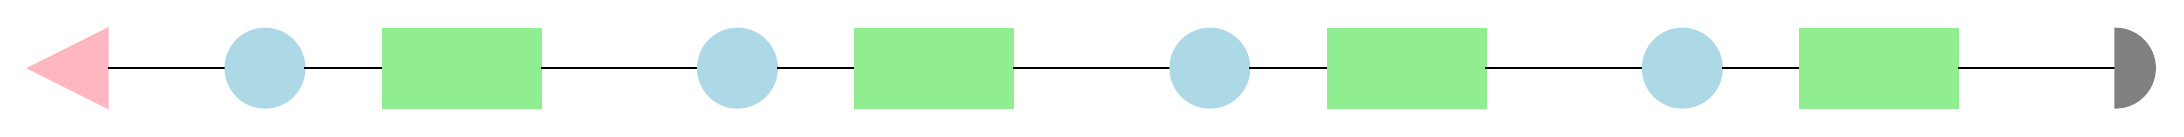
\begin{tikzpicture}

    % Define colors
    \definecolor{pastelblue}{RGB}{173,216,230}
    \definecolor{pastelyellow}{RGB}{255,255,204}
    \definecolor{pastelgreen}{RGB}{144,238,144}
    \definecolor{pastelred}{RGB}{255,182,193}

    \filldraw[pastelred, thick] (-3,0) -- (-2,0.5) -- (-2,-0.5) -- cycle;
    \draw[thick] (-2,0) to (0,0);

    \filldraw[pastelblue, thick] (0,0) circle(0.5);
    \draw[thick] (0.5,0) to (1.5,0);
    \filldraw[pastelgreen, thick] (1.5,0.5) rectangle (3.5,-0.5);

    \draw[thick] (3.5,0) to (5.5,0);

    \filldraw[pastelblue, thick] (6,0) circle(0.5);
    \draw[thick] (6.5,0) to (7.5,0);
    \filldraw[pastelgreen, thick] (7.5,0.5) rectangle (9.5,-0.5);

    \draw[thick] (9.5,0) to (11.5,0);

    \filldraw[pastelblue, thick] (12,0) circle(0.5);
    \draw[thick] (12.5,0) to (13.5,0);
    \filldraw[pastelgreen, thick] (13.5,0.5) rectangle (15.5,-0.5);

    \draw[thick] (15.5,0) to (17.5,0);

    \filldraw[pastelblue, thick] (18,0) circle(0.5);
    \draw[thick] (18.5,0) to (19.5,0);
    \filldraw[pastelgreen, thick] (19.5,0.5) rectangle (21.5,-0.5);

    \draw[thick] (21.5,0) to (23.5,0);
    \filldraw[gray, thick] (23.5,0.5) arc (90:-90:0.5) -- cycle;


\end{tikzpicture}

\end{document}

